\documentclass{beamer}
\usepackage[latin1]{inputenc}

\usepackage{graphicx}
\usepackage{listings}
\lstset{basicstyle=\tiny}

\newcommand{\bra}[1]{\langle #1|}
\newcommand{\ket}[1]{|#1\rangle}
\newcommand{\braket}[2]{\langle #1|#2\rangle}

\setlength{\parskip}{\baselineskip}

\usetheme{Warsaw}
\title[I/O and Memory]{I/O and Memory. \\ Experiences from Computation Chemistry}
\author{Andrey Asadchev}
\institute{VT.edu}

\begin{document}

\begin{frame}
  \titlepage
\end{frame}

\begin{frame}{Mountain Creek in Western Virginia}
\begin{figure}[here]
\begin{center}
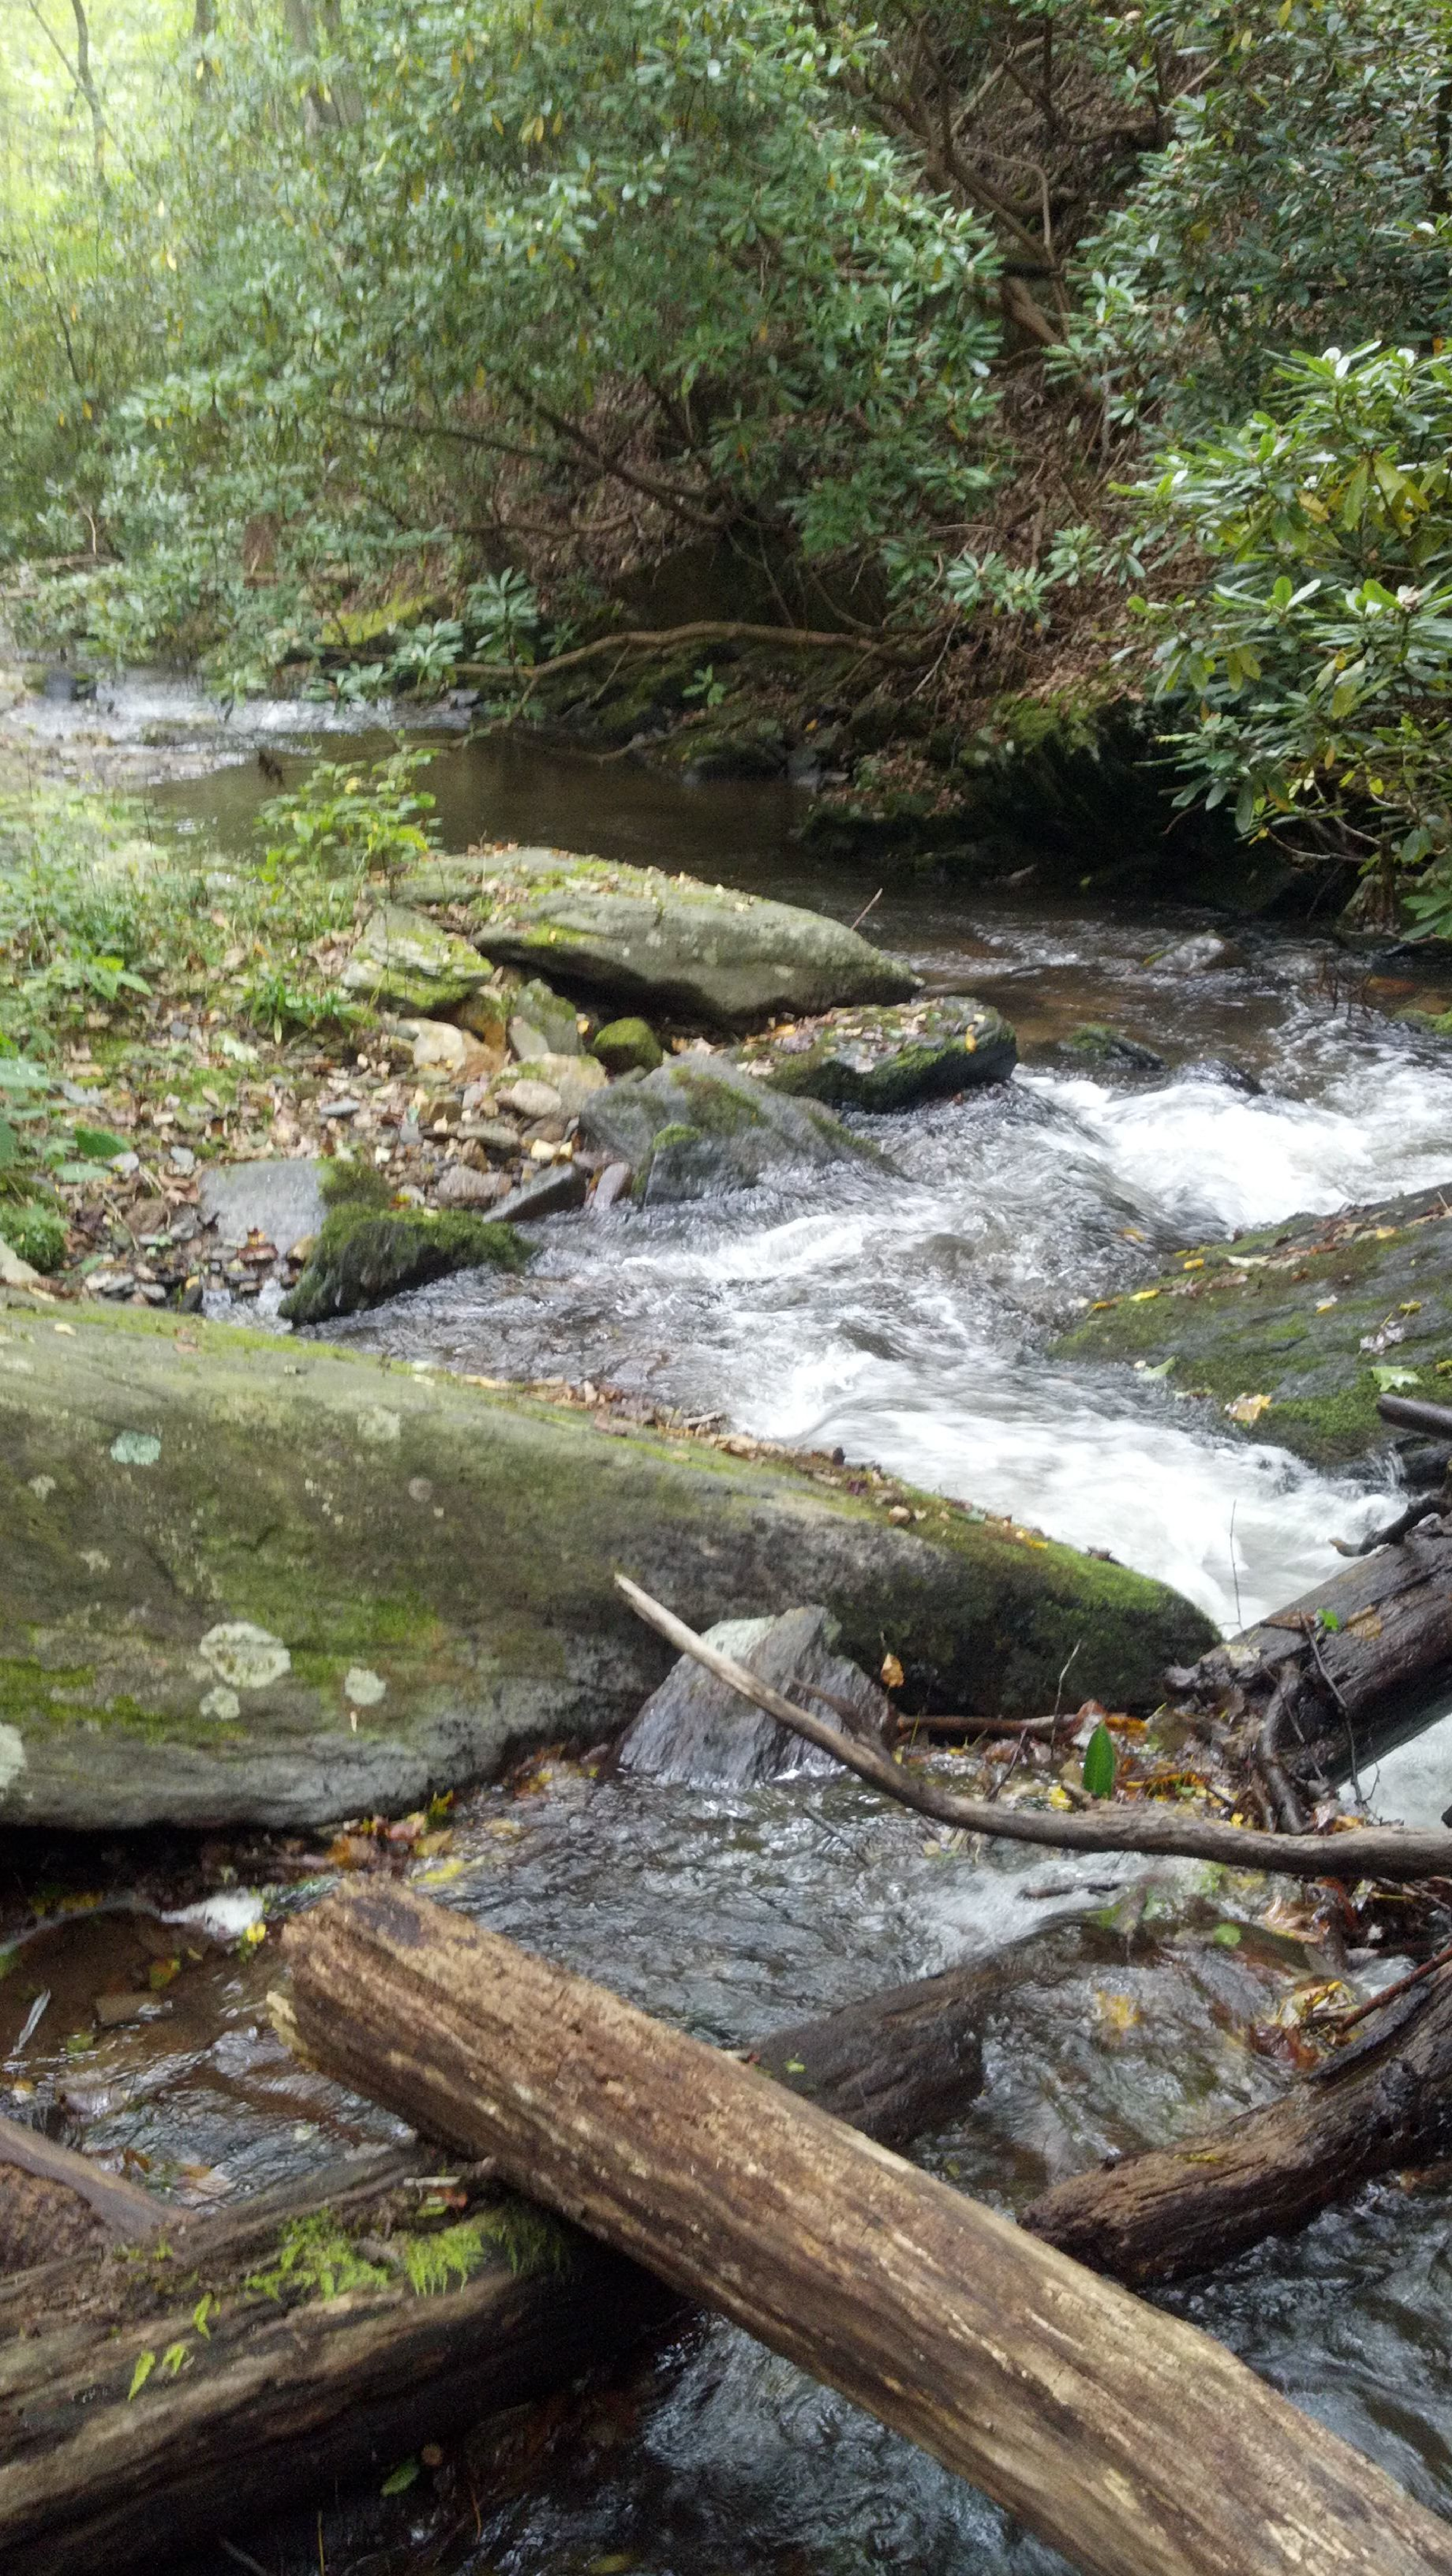
\includegraphics[scale=0.07]{va.pdf}
\end{center}
\end{figure}
\end{frame}

\begin{frame}{Forewarning}
To keep the presentation short and accessible to a wide audience,
many theoretical details are glossed over and/or represented in simplified manner.
\end{frame}

\begin{frame}{A Very Brief Overview of Computation Chemistry}
\begin{itemize}
\item The goal is to obtain energies and properties of a molecule from {\em first principles}
  ie via the Schrodinger equation $H \Psi = E \Psi$
\item Most systems have no closed-form solution and must rely on approximations.
\item The wavefunction $\Psi$ in typically represented in terms of $N$ atomic basis functions $\chi$.
\item The wavefunction is then a linear combination, $\psi_i = \sum_b^{N} c_{ib} \chi_b$
\item Coefficients are optimized so as to minimize the energy.
\item The most common {\em first-order} method is Hartree-Fock (HF), which is an iterative method.
\item In its common formulation, $FC = EC$ HF requires computing so called two-electron integrals
  and diagonalizing the operator (eigenvalue problem)
\end{itemize}
\end{frame}

\begin{frame}{First I/O Bottleneck}
\begin{itemize}
\item The two-electron integrals do not change during the iterative HF steps.
\item They maybe precomputed and reused, as was done in the early days.
\item However, there are $N^4$ integrals, as opposed to $F$ operator which is $N^2$,
  and even with the modest basis of say 750 basis functions, the storage is 2.5TB
\item It was quickly realized that re-computing integrals on the fly was way more efficient.
\item This approach to HF is called direct HF.
\item In chemistry parlance, {\em direct} oftentimes refers to methods which recompute the intermediates.
\end{itemize}
\end{frame}

\begin{frame}{Past Hartree-Fock}
\begin{itemize}
\item The common wisdom is that HF about recovers 99\% of {\em total} energy and produces fairly accurate geometries.
\item The 1\% that Hartree-Fock leaves out is what is called the correlation energy.
\item The properties associated with that 1\% is what theorists usually seek.
\item The electron correlation methods try to recover that 1\% from the HF wavefunction.
\end{itemize}
\end{frame}

\begin{frame}{Electron correlation methods}
\begin{itemize}
\item Moller-Plesset Second Order (MP2) is a fairly cheap method, scales as $N^5$.
\item Coupled-Cluster (CC) methods are consider the best, but scale as $N^6$ and beyond.
\item Configuration Interaction (CI) method gives the exact result (within the limits of the basis set) but scales as $N!$
\item All electron correlation methods involve manipulations of large datasets, on the order of gigabytes and terabytes.
\item Over the years researcher developed methods to decrease storage and computation, for example resolution-of-identity (RI), density-fitting (DF), and other methods.  The cutting edge are the PNO methods (in my opinion).
\end{itemize}
\end{frame}

\begin{frame}{The Problem with Memory and I/O}
\begin{itemize}
\item The implementations typically try to store work data in memory,
  either on node or distributed across the cluster.
\item That limits the range of machines a user can utilize and pushes a finite resource (as opposed to infinite time).
\item Some data access must be fast, eg if the data is accessed in innermost loops or must be accessed in non-contiguous blocks.
\item Typically one would use various tricks such as pre-fetching, loop blocking, and computation/communication overlap to hide/decrease access latency.
\item But algorithms can be re-arranged and modified so that most of data is accessed only once per outer loop, in large blocks.
\item In that case, the data can be stored on the filesystem with minimal overhead.
\end{itemize}
\end{frame}

\begin{frame}{CI}
\begin{itemize}
\item CI is given as $\ket{\Psi} = c_0 \bra{\Phi_0} + \sum{c_i^a \bra{\Phi_i^a} } +  ..$
\item In essence, we want to consider every possible replacement from the reference.
\item In other words, we want to ``distribute'' $N$ electrons among $K$ orbitals:
 there are ${K \choose N_\alpha}$ alpha and ${K \choose N_\beta}$ beta arrangements (strings).
\item A particular configuration will be an alpha-beta string pair (determinant) and we want to consider ALL pairs.
\item The entire Hamiltonian is square the number of ALL pairs!!!
\item Only for smallest of values can the Hamiltonian be evaluated in full and diagonalized.
\item For anything larger, the CI roots (eigenvalues) and coefficient vectors (CI vectors)
  need to be evaluated iteratively (Davidson method)
\end{itemize}
\end{frame}

\begin{frame}{CI}
\begin{itemize}
\item The strings can be represented with 0s (empty orbitals) and 1s (electrons).
\item This leads to a bit strings representation, eg. $101 .. 100$.
\item For example $K = 4, N = 2$ configuration will generate $1100, 1010, 1001, 0110, 0101, 0011$
\item Bit strings can be indexed and manipulated efficiently using bit operators and hardware instruction: {\tt \&, >>, POPCNT, ...}.
\item The entire string list can sorted lexicographically and indexed using minimal perfect hash: \\
  {\tt hash(s) = Upper[16 >> s] + Lower[0xFFFF  \& s]}
\end{itemize}
\end{frame}


\begin{frame}{The three CI parts}
\begin{itemize}
\item The three types of CI excitations are alpha-alpha, beta-beta, and simultaneous alpha-beta.
\item Those are commonly referred to as $\sigma_1, \sigma_2, \sigma_3$. \\
\begin{align*}
\sigma_1(a,b) =& \sum_{b'} \sum_{ij}   { \bra{b} E_{ij}^{\beta} \ket{b'} h'_{ij} C(a,b') } + \\
& \frac{1}{2} \sum_{b'} \sum_{ijkl} { \bra{b} E_{ij}^{\beta} \ket{b'} \bra{b'} E_{kl}^{\beta} \ket{b''} (ij|kl) C(a,b') }
\\
\sigma_2(a,b) =&
  \sum_{a'} \sum_{ij}   { \bra{a} E_{ij}^{\alpha} \ket{a'} h'_{ij} C(a',b) } + \\
& \frac{1}{2} \sum_{a'} \sum_{ijkl} { \bra{a} E_{ij}^{\alpha} \ket{a'} \bra{a'} E_{kl}^{\alpha} \ket{a''} (ij|kl) C(a',b) }
 \\
\sigma_3(a,b) =& \frac{1}{2}\sum_{a'b'} \sum_{ijkl} {
  \bra{a} E_{ij}^{\alpha} \ket{a'} \bra{b} E_{kl}^{\beta} \ket{b'} (ij|kl) C(a',b')
}
\end{align*}
\end{itemize}
\end{frame}

\begin{frame}{The CI Dimensions}
 To give an idea of CI datasets
\begin{itemize}
\item (16 16) CI (16 orbitals, 8 alpha, 8 beta): 12,870 strings, 165 million determinants.  $C, \sigma$ each require 1.3GB
\item (20 20) CI (20 orbitals, 10 alpha, 10 beta): 184,756 strings, 34 billion determinants.  $C, \sigma$ each require 273GB
\item (21 20) CI (21 orbitals, 10 alpha, 10 beta): 352,716 strings, 124 billion determinants.  $C, \sigma$ each require 995GB.
\item Moreover, previous $C$ vectors must be retained in the Davidson expansion.
\end{itemize}
\end{frame}

\begin{frame}{Overall CI algorithm}
\begin{itemize}
\item CI algorithm can be broken down into two parts:  \\
  the calculation of $\sigma$ vector, $\sigma = \mathbf{H} c$ and Davidson iteration
\item $\sigma$ computation is computationally and I/O heavy, especially $\sigma_3$ part
\item The Davidson step is a straightforward linear algebra, primarily dot products and scaling.
\item The data for the Davidson step can be made local to each node.  There is no data transfer required other than the reduction of partial dot products. 
  Very straightforward to implement to utilize filesystem to the max.
\item Since the data will be local to a node, the I/O will scale with the number of nodes.
\end{itemize}
\end{frame}

\begin{frame}{Sigma 1/2}
\begin{itemize}
\item Sigma 2 computations can be formulated as
  $\sigma(a,b) = \sum_{b'} F(b \rightarrow b') C(a,b')$, where $F(b \rightarrow b')$
  depends only on beta string excitation and corresponding one- and two- electron integrals.
  Sigma 1 for $a'$ is defined similarly
\item In the closed-shell case, $C(a,b)$ is symmetric and $\sigma_1(a,b) = -1^{S} \sigma_2(b,a)$
\item The expression can be rewritten as $\sigma(b,a) = \sum_{b'} F(b \rightarrow b') C(b',a)$
\item In other words, to compute column $a$ of $\sigma$, we only need the corresponding $C$ column
\item Very easy to parallelize and to distribute data, \\
  distribute data column-wise and operate on local columns of $C$ and $\sigma$
\item In case of open-shell, transpose either matrix/vector between the two steps
\end{itemize}
\end{frame}

\begin{frame}[fragile]{Sigma 3}
\begin{itemize}
\item $\sigma_3(a,b) = \sum_{a'b'} F(a \rightarrow a', b \rightarrow b') C(a',b')$, 
\item Notice the big difference from earlier $\sigma$,
  neither rows nor columns ``match'' between $\sigma$ and $C$.
  That means a lot of I/O.
\item Lets say we need to compute a beta column $111000$.  Allowed excitations are  \\
$111000, 110100, 110010, 110001, 101100, ...$. \\
All those columns will need to be loaded.
\item What about a beta column $110100$?  Allowed excitations are \\
$111000, 110100, 110010, 110001, 101100, ...$. \\
That's a lot of overlap with a beta column $111000$.
\item I/O overhead can be hidden by computing a block of beta columns at a time.
\end{itemize}
\end{frame}

\begin{frame}[fragile]{Sigma 3}
 The general approach
\begin{itemize}
\item Pick a block of beta columns to compute.
\item For each of those beta strings, generate all valid excitations.
\item Sort excitation list
\item Loop over excitation list in blocks (list may have gaps)
\item Load $C(:,b')$ corresponding to that block
\item Evaluate $\sigma(:,b)$ columns corresponding to $C(:,b')$ block. \\
  Those $\sigma(:,b)$ columns aren't necessarily contiguous!
\item The I/O part is (kinda) taken care of.
\end{itemize}
\end{frame}

\begin{frame}[fragile]{Sigma 3}
  There is a lot of indexing involved in 
  $\sigma_3(a,b) = \sum_{a',b'} E_{ij}^{aa'} E_{kl}^{bb'} (ij|kl) C(a',b')$ \\
  We need to get valid excitations, phase factors, orbitals that are swapped, etc.
  One could try a few tricks.
\begin{itemize}
\item Make a subcopy of $(ij|kl)$, lets call it $(ij|b')$, corresponding to
  $b \rightarrow b'$ excitations in the block.
\item Apply $b \rightarrow b'$ phase factors to $(ij|b')$.
\item Now the $b'$ dimension no longer requires indirect indexing: \\
  $\sigma_3(a,b) = \sum_{a',b'} E_{ij}^{aa'} (ij|b') C(a',b')$.
\item Assuming column-major storage, need to transpose matrices.
\item There is no way to get rid of alpha indexing but
  for each alpha phase/index lookup there will be a block of vectorizable operations.
\end{itemize}
\end{frame}


\begin{frame}[fragile]{Performance}
Sample computation, 124,408,576,656 determinants, 64 nodes x 16 cores, 1024 total cores.
\begin{itemize}
\item Overall $\sigma$ time about 4300s, a bit over an hour.
\item $\sigma_{1+2}$ takes about 1300s
\item Out of that, $\sigma_{1+2}$ {\em kernel} accounts for about 50\%.
\item $\sigma_{1+2}$ I/O (read and write) is about 10\%.
\item $\sigma_{3}$ takes about 3000s, runs at about 20\% of max CPU rate.
\item Out of that, the {\em kernel} accounts for about two thirds of time.
\item I/O overhead isn't bad, on the order of 10\% but in-memory data reordering is rather expensive
\item With one-two expansion vectors, Davidson overhead is low, around 10\% of total wall time.
  Davidson wall time increases with the number of expansion vectors.
\end{itemize}
\end{frame}

\begin{frame}[fragile]{Further improvements}
Lexicographical ordering isn't the best.
\begin{itemize}
\item Consider the case of $\sigma_3$, for a rank $R$ string, only $R-1, R, R+1$ subset is needed.
\item With lexicographical ordering, the ranks are all over the place and I/O is not localized
\item Instead, (stable) sort the lexicographically ordered strings by their ranks.
\item Now the I/O will be limited only to neighbouring blocks $R-1, R, R+1$
\end{itemize}
\end{frame}

\begin{frame}[fragile]{Programming Aspects}
The object hierarchy is three-tiered
\begin{itemize}
\item In-core {\tt Tensor, Matrix, Vector}, derived from {\tt Eigen} library.
\item Distributed {\tt Array}, implemented in terms of various backends, eg ARMCI, HDF5, MPI, etc.
\item {\tt File} and file objects {\tt Dataset, Group, ...} implemented on top of HDF5.
\item Each object has {\tt range} access operators to give sub-block access.
\item In-core objects can be read/written to/from {\tt Array} and file objects.
\item {\tt Array} object can be read/written to/from file objects.
\end{itemize}
\end{frame}

\begin{frame}[fragile]{Example}
\begin{verbatim}
// create/open file
File file = File("file.h5");
// create dataset
File::Dataset<double> ds(file, "my dataset", dims);
Matrix a = Matrix::Random(m,n); // create some matrices
Matrix b = Matrix::Random(m-1,n-1);
ds << a; // write matrix to dataset
ds(range(0,m-1), range(0,n-1) >> b; // read subset
...
// create array, comm is MPI communicator
Array<double> array("my array", dims, comm);
a(0,2) = 3.14;
// write to distributed array
array(range(1,m), range(1,n)) << a;
\end{verbatim}
\end{frame}


\begin{frame}[fragile]{Questions.}
Questions.
\end{frame}


\end{document}
